\documentclass[11pt]{exam}
\usepackage[margin=1in]{geometry}
\pagestyle{plain}
\usepackage{amsmath,amsfonts,amssymb,amsthm,enumerate}
\usepackage{multicol}
\usepackage[]{graphicx}
\usepackage{hyperref}
\usepackage{tikz}
\usepackage{pgfplots}
\usepackage{subfigure}
\usepackage[final]{pdfpages}


\everymath{\displaystyle}

\addtolength{\footskip}{2\baselineskip} % to lower the page numbers
\title{\vspace{-0.75in} Math 115 \\ Worksheet Section 6.1}
\date{}


% \theoremstyle{definition}
% \newtheorem{problem}{Problem}
\renewcommand{\questionlabel}{\textbf{Problem~\thequestion.}}
%\printanswers

\begin{document}
\maketitle
\vspace{-0.5in}
\noindent The function $F(x)$ is an antiderivative of $f(x)$ if \fillin[\(F'(x)
= f(x)\)][4cm].

\vspace{0.5cm}

\noindent If $F(x)$ is an antiderivative of the differentiable function $f(x)$,
	\begin{enumerate}[(a)]
		\item if $f$ is positive on an interval, then $F$ is \fillin[increasing][4cm] on that interval.
		\item if $f$ is increasing on an interval, then $F$ is
                  \fillin[concave up][4cm] on that interval.
	\end{enumerate}
\begin{questions}
  \question For each of the given functions $f$, sketch the graphs of its antiderivatives $F$, $G$, $H$ and $K$ such that $F(0)=0$, $G(0)=1$, $H(0)=2$ and $K(0)=-2$.
\begin{multicols}{2}
\begin{enumerate}[(a)]
\item $f$ is the constant function $f(x)=0$.	
\item $f$ is the constant function $f(x)=1$.	
\end{enumerate}
\end{multicols}
\begin{minipage}{0.5\linewidth}
  (c)
  \begin{tikzpicture}[scale=0.8]
    \draw[->] (-3,0) -- (3,0) node[right] {$x$}; \draw[->] (0,-3) --
    (0,3) node[above] {$y$};
    \draw[scale=0.5,domain=-2:2,smooth,variable=\x,thick,magenta] plot
    ({\x},{2*\x}); \node [above] at (2,2) {$y=f(x)$}; \foreach\x
    in{-2,-1,1,2}{
      \draw(\x,0)--(\x,-0.1)node[below,font=\small]{$\x$};};
    \foreach\y in{-1,1,2}{
      \draw(-0.1,\y)--(0,\y)node[left,font=\small]{$\y$};}; \node
    [below] at (-0.2,0) {$0$};
  \end{tikzpicture}
\end{minipage}
\begin{minipage}{0.5\linewidth}
  (d) 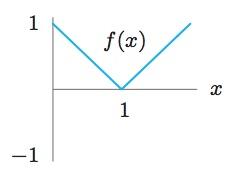
\includegraphics[width=2.5in]{no7.jpg}
\end{minipage}
\begin{solution}
  \begin{multicols}{2}
    \begin{enumerate}[(a)]
    \item 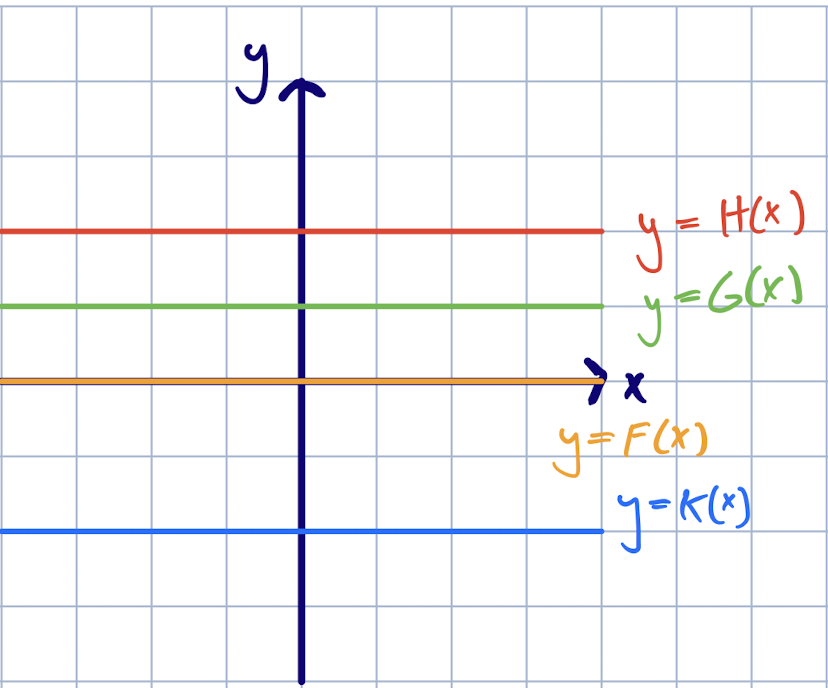
\includegraphics[scale=0.4]{1a}
    \item 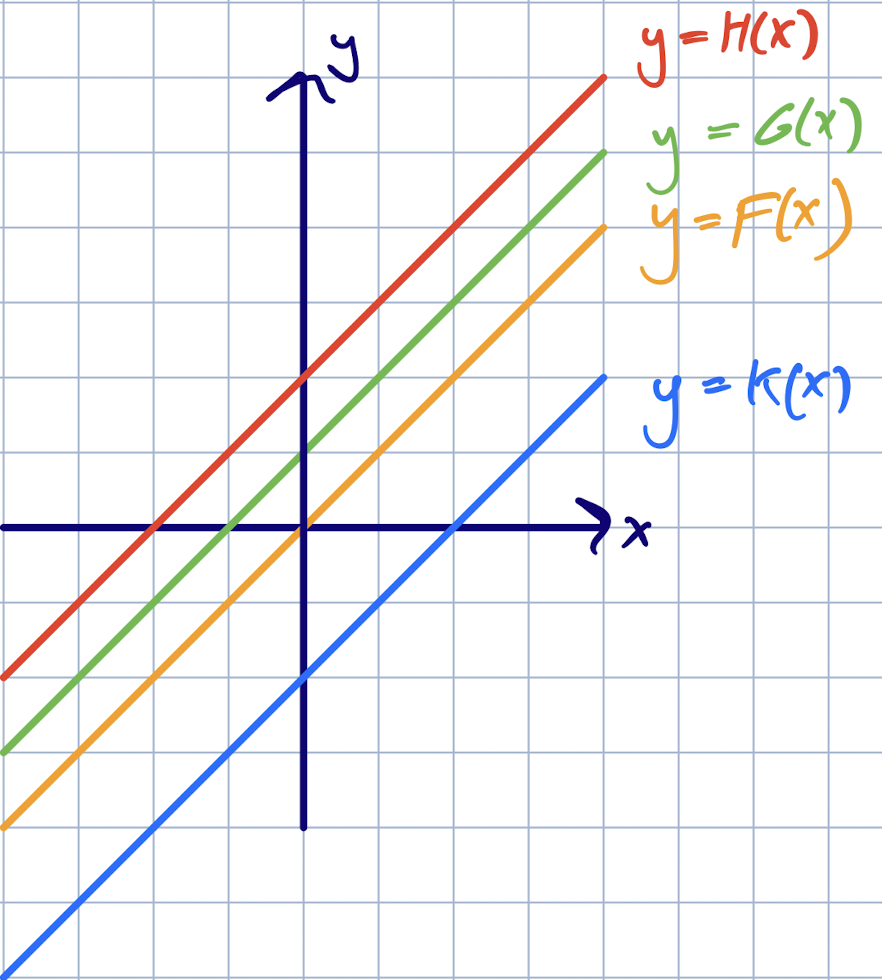
\includegraphics[scale=0.4]{1b}
    \item 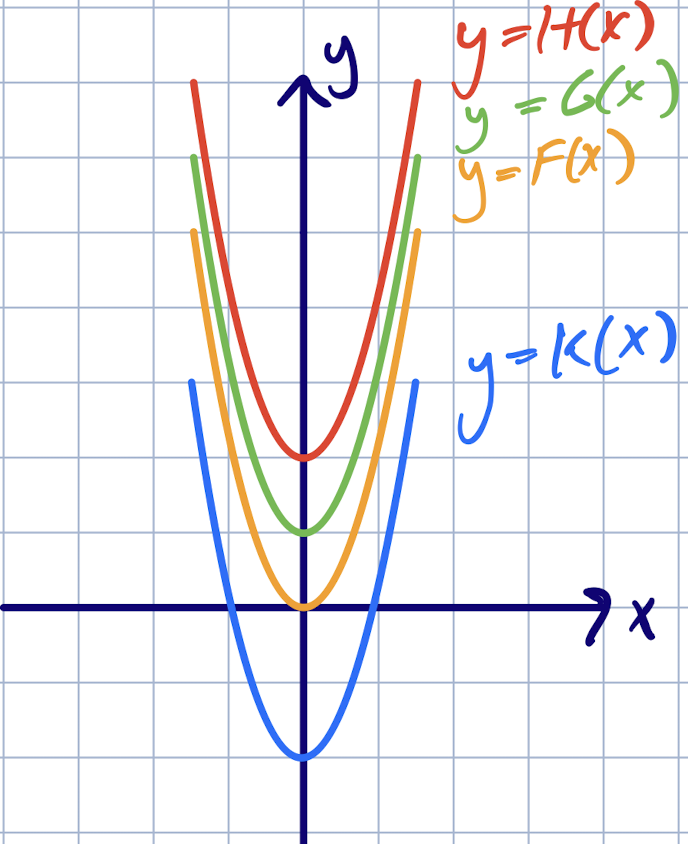
\includegraphics[scale=0.4]{1c}
    \item 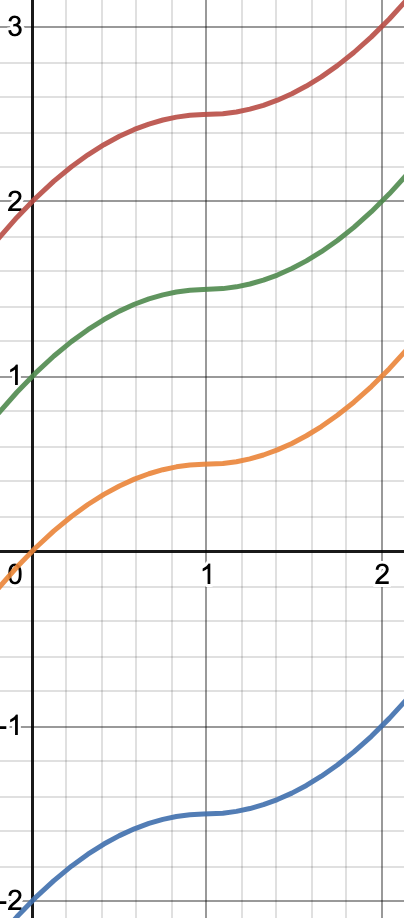
\includegraphics[scale=0.7]{1d}
    \end{enumerate}
  \end{multicols}
\end{solution}
\question Let \(F(x)\) be the antiderivative of \(f(x)\).
  \begin{parts}
  \part If \(\int_2^5 f(x) dx = 4\) and \(F(5) = 10\), find \(F(2)\).
  \part If \(\int_0^{100} f(x) dx = 0\), what is the relationship
    between \(F(100)\) and \(F(0)\)?
  \end{parts}
  \begin{solution}
    \begin{enumerate}[(a)]
    \item We know \(4 = \int_2^5 f(x) dx = F(5)-F(2) = 10-F(2)\), so
      \(F(2) = 6\).
    \item This tells us \(F(100)-F(0) = 0\), so \(F(100) = F(0)\).
    \end{enumerate}
  \end{solution}
\question Assume \(f'\) is given by the graph below. Suppose \(f\) is
  continuous and that \(f(0) = 0\). 

  \begin{minipage}{0.5\linewidth}
    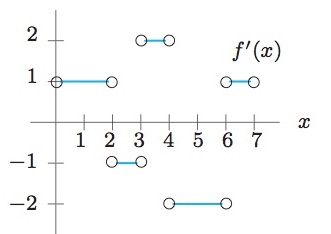
\includegraphics[scale=0.4]{no33}
  \end{minipage}
  \begin{minipage}{0.5\linewidth}
    \begin{enumerate}[(a)]
    \item Find \(f(3)\) and \(f(7)\).
    \item Find all \(x\) with \(f(x) = 0\).
    \item Sketch a graph of \(f\) over \(0 \leq x \leq 7\).
    \end{enumerate}
  \end{minipage}
  \begin{solution}
    \begin{enumerate}[(a)]
    \item We know that \(\int_0^3 f'(x) dx = f(3)-f(0) = f(3)\) since
      \(f(0) = 0\). From the graph, we can add up the signed area to
      see \[
        f(3) = \int_0^3 f'(x) dx = 2-1 = 1
      \]
      Similarly, we can compute \[
        f(7) = \int_0^7 f'(x) dx = 2-1+2-4+1 = 0
      \]
    \item Besides \(f(0)\) and \(f(7)\), we compute that \[
        f(5.5) = \int_0^{5.5} f'(x) dx = 2-1+2-2(1.5) = 0
      \]
      Thus, \(x=0,5.5,7\) is the final answer.
    \item 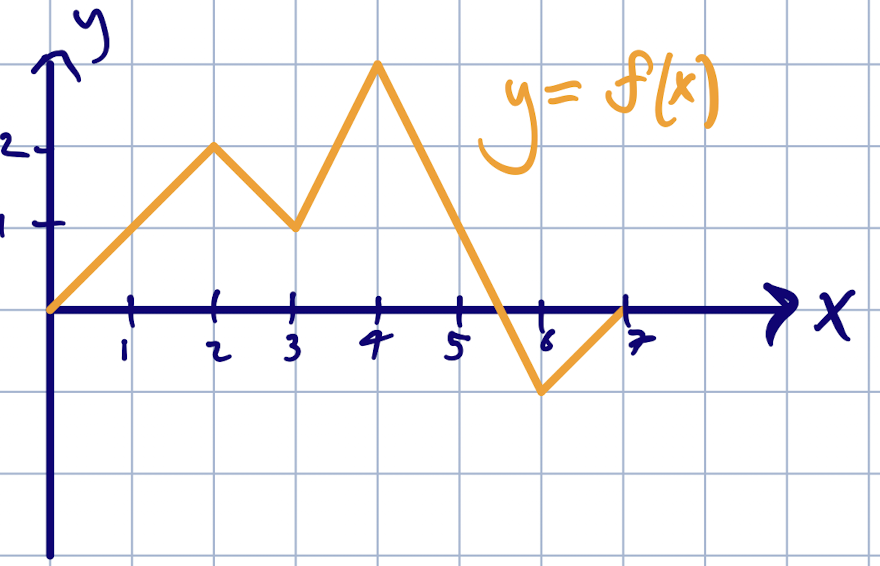
\includegraphics[scale=0.5]{3c}
    \end{enumerate}
  \end{solution}
\question \,

  \begin{minipage}{0.5\linewidth}
    The function $g$ is defined on the interval $[-2,2]$ and has
    $g(-1)=1$. The graph of its derivative $g'(x)$ is given. Sketch
    the graph of $g$.
  \end{minipage}
  \begin{minipage}{0.5\linewidth}
    \begin{tikzpicture}[yscale=0.5]
      \draw[->] (-3,0) -- (3,0) node[right] {$x$}; \draw[->] (0,-2) --
      (0,3) node[above] {$y$};
      \draw[scale=0.5,domain=-4:0,smooth,variable=\x,blue,thick] plot
      ({\x},{0});
      \draw[scale=0.5,domain=0:4,smooth,variable=\x,thick,blue] plot
      ({\x},{\x}); \node [above] at (2,2) {$y=g'(x)$}; \foreach\x
      in{-2,-1,1,2}{
        \draw(\x,0)--(\x,-0.1)node[below,font=\small]{$\x$};};
      \foreach\y in {1,2}{
        \draw(-0.1,\y)--(0,\y)node[left,font=\small]{$\y$};}; \node
      [below] at (-0.2,0) {$0$};
    \end{tikzpicture}
  \end{minipage}
  \begin{solution}
   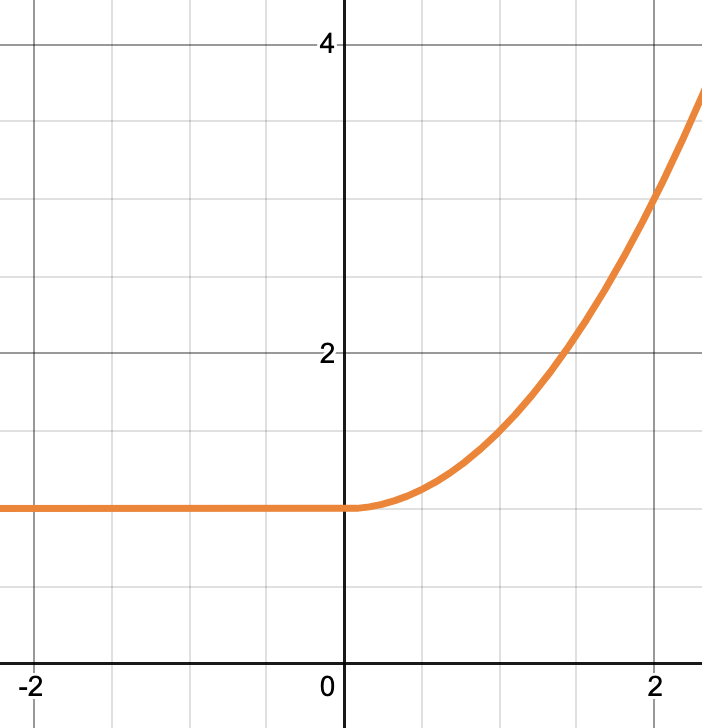
\includegraphics[scale=0.5]{4}
  \end{solution}
  \pagebreak
\question The graph of \(\frac{dy}{dt}\) against \(t\) is below. The
  three shaded regions each have area \(2\). If \(y=0\) when \(t=0\), 
  draw the graph of \(y\) as a function of \(t\), labeling the known
  \(y\)-values, maxima and minima, and inflection points. Mark \(t_1,
  t_2, \ldots, t_5\) on the \(t\) axis.

  \begin{center}
    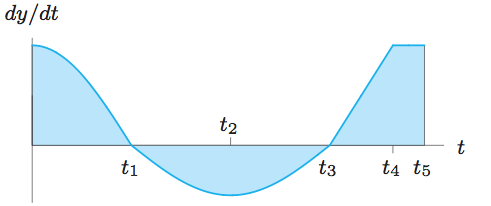
\includegraphics[scale=0.5]{no17}
  \end{center}
  \begin{solution}
    \begin{center}
      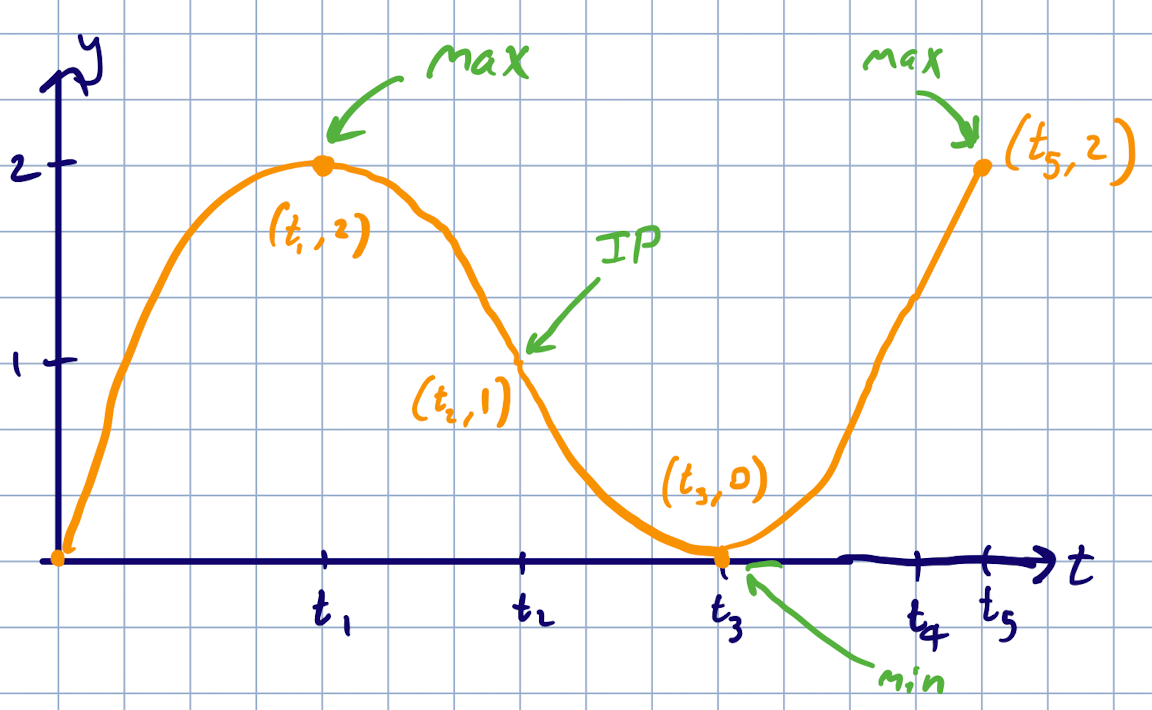
\includegraphics[scale=0.5]{5}
    \end{center}
  \end{solution}
\question The Quabbin Reservoir in the western part of Massachusetts
  provides most of Boston's water. The graph below represents the flow
  of water in and out of the Quabbin Reservoir throughout 2007.
  \begin{parts}
  \part Sketch a graph of the quantity of water in the reservoir as a
    function of time. 
  \part When, in the course of 2007, was the quantity of water in the
    reservoir largest? Smallest? Mark and label these points on the
    graph you drew in part (a). 
  \part When was the quantity of water increasing most rapidly?
    Decreasing most rapidly? Mark and label these times on both graphs.
  \end{parts}
  \begin{center}
    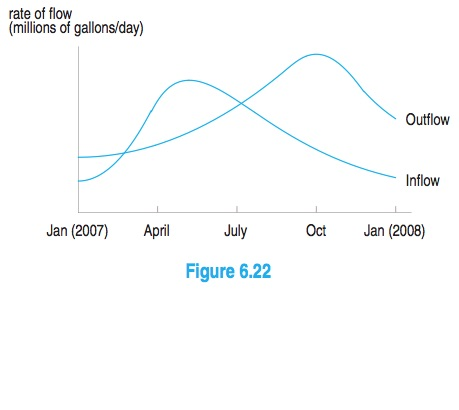
\includegraphics[scale=0.5]{no35graph}
  \end{center}
  \vspace{-1in}
  \begin{solution}
    \begin{enumerate}[(a)]
    \item 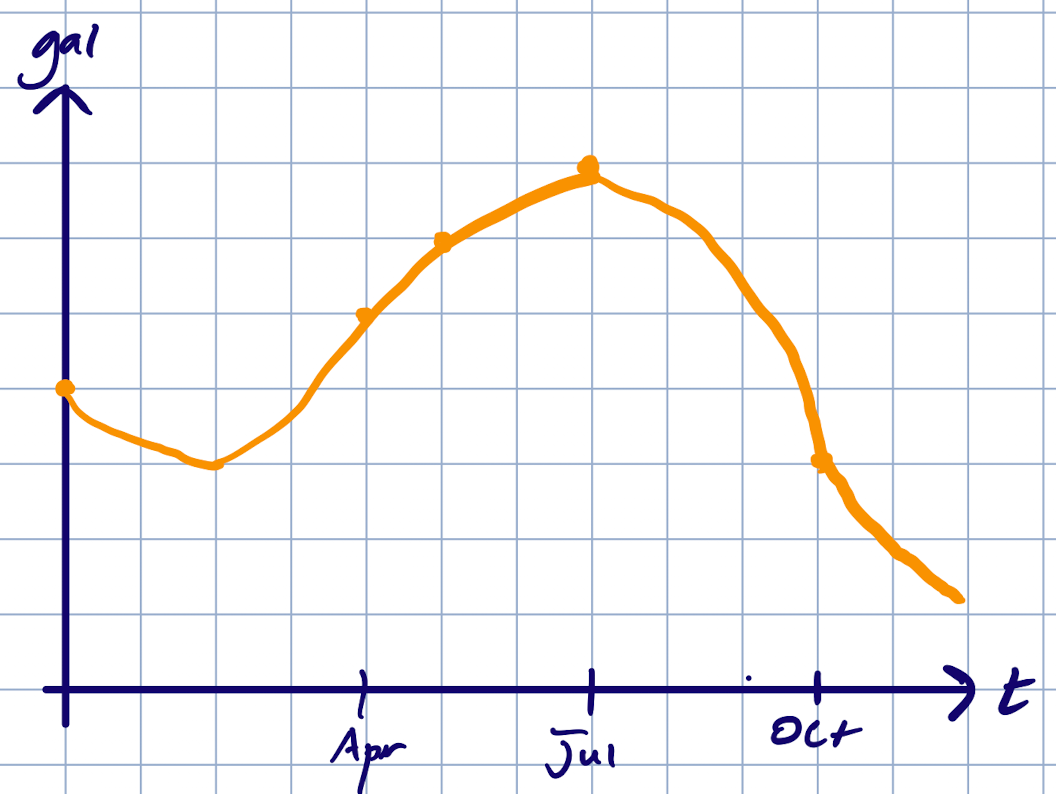
\includegraphics[scale=0.5]{6a}
    \item It was the largest in July and the smallest in January 2008.
    \item It was increasing the fastest in May and decreasing the
      fastest in October.
    \end{enumerate}
  \end{solution}
\question (Fall 2013 Final Exam) % problem 3
The function $g(t)$ is the volume of water in the town water tank, in thousands of gallons, $t$ hours after 8 A.M. A graph of $g'(t)$ is shown below. Note that $g'(t)$ is a piecewise-linear function. Suppose that $g(3) = 1$.

\begin{minipage}{0.5\linewidth}
  \begin{center}
    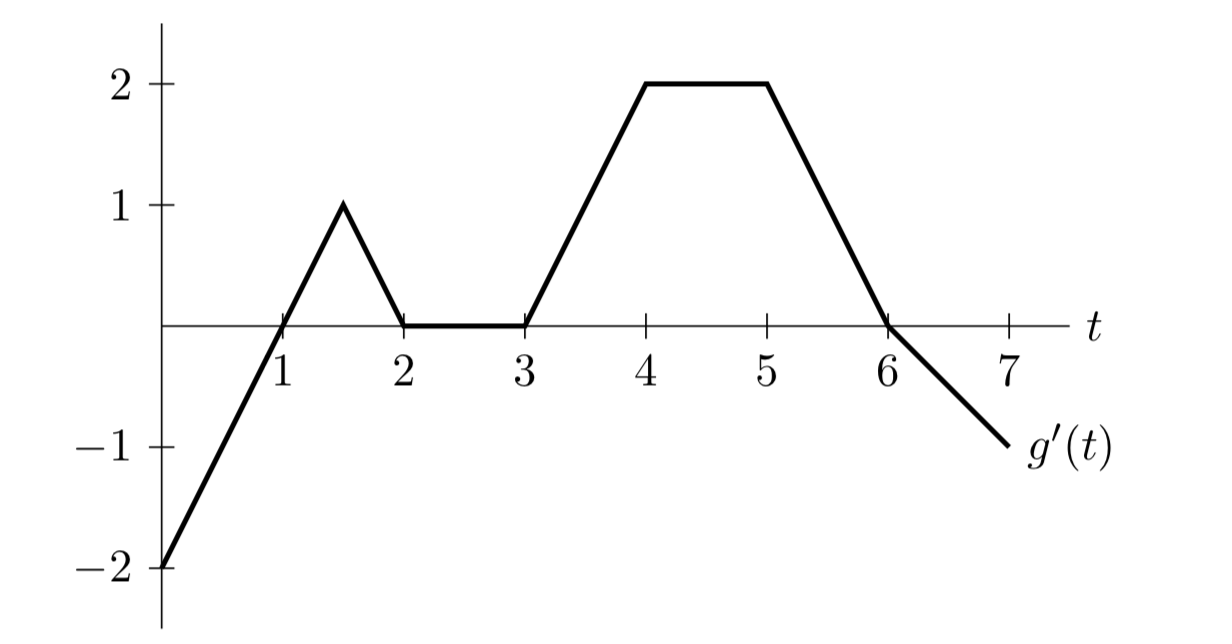
\includegraphics[scale=0.4]{graphg}
  \end{center}
\end{minipage}
\begin{minipage}{0.5\linewidth}
  \begin{enumerate}[(a)]
  \item Write an integral which represents the average rate of change,
    in thousands of gallons per hour, of the volume of water in the
    tank between 9 A.M. and 1 P.M. Compute its exact value.
  \item At what time does the tank have the most/least water in it?
  \item Sketch a graph of $g(t)$ and give both coordinates of the
    point on the graph at $t = 7$.
  \end{enumerate}
\end{minipage}
\begin{solution}
  See \href{https://dhsp.math.lsa.umich.edu/exams/115exam3/f13/s3.pdf}{https://dhsp.math.lsa.umich.edu/exams/115exam3/f13/s3.pdf}
\end{solution}
\question (Fall 2014 Final Exam) %problem 4
	A portion of the graph of $y = f(x)$ is shown below.	 The area of the region $A$ is $3$, and the area of the region $B$ is $3$. Let $F(x)$ be the continuous antiderivative of $f(x)$ with $F(0) = 1$ whose domain includes the interval $-6 \leqslant x \leqslant 4$.
        \begin{center}
	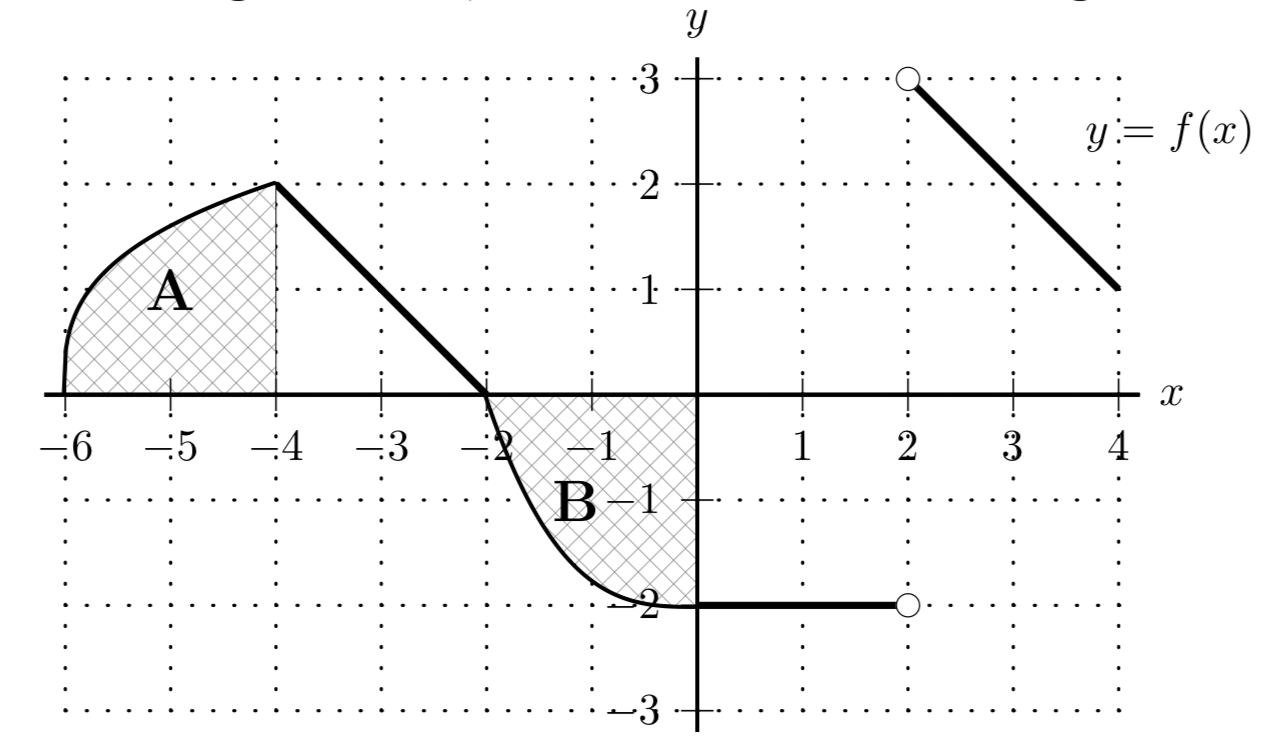
\includegraphics[scale=0.45]{graphf}
        \end{center}
	\begin{enumerate}[(a)]
		\item For what value(s) of $x$ with $-6 < x < 4$ does $F(x)$ have local extrema?
		\item Sketch the graph of $y = F(x)$ on the interval $-6 \leqslant x \leqslant 4$.
Pay close attention to the following:
\begin{itemize}
\item the value of $F(x)$ at each of $x = -6, -4, -2, 0, 2, 4$;
\item where $F$ is/is not differentiable;
\item where $F$ is increasing/decreasing/constant;
\item the concavity of the graph of $y = F (x)$.
\end{itemize}
\end{enumerate}
\begin{solution}
  See \href{https://dhsp.math.lsa.umich.edu/exams/115exam3/f14/s4.pdf}{https://dhsp.math.lsa.umich.edu/exams/115exam3/f14/s4.pdf}
\end{solution}
\question (Fall 2016 Final Exam) % problem 11
	A portion of the graph of $k$ is shown below. Note that for $3 < x < 5$, the graph of $k(x)$ is a portion of the graph obtained by shifting $y=x^2$ three units to the right. Let $K(x)$ be a continuous antiderivative of $k$ passing through the point $(-1,1)$.
	\vspace{-0.5em}
        \begin{center}
          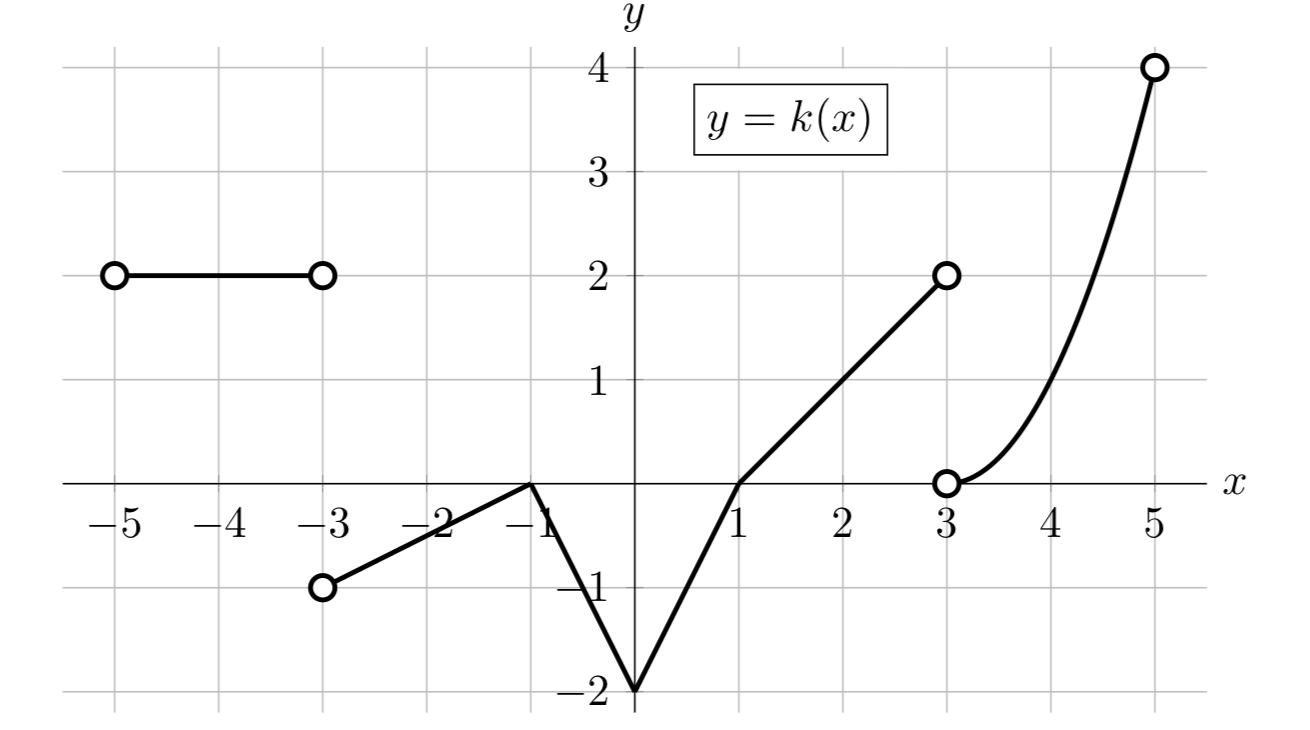
\includegraphics[scale=0.45]{graphk}
        \end{center}
	\vspace{-2em}
	\begin{enumerate}[(a)]
		\item Use the graph to complete the table with exact values of $K$.
		$$\begin{array}{|c||c|c|c|c|c|c|c|}
	\hline
	x & -5 & -3 & -1 & 1 & 3 & 5 \\
	\hline
	K(x) & & & & & & \\
	\hline
	\end{array}$$
		\item Sketch a detailed graph of $y = K(x)$ for $-5 < x < 5$. Pay close attention to the following:
\begin{itemize}
	\item where $K(x)$ is and is not differentiable,
	\item the values of $K(x)$ you found in the table above,
	\item where $K(x)$ is increasing/decreasing/constant, and the concavity of $K(x)$.
\end{itemize}
	\end{enumerate}
        \begin{solution}
          See \href{https://dhsp.math.lsa.umich.edu/exams/115exam3/f16/s11.pdf}{https://dhsp.math.lsa.umich.edu/exams/115exam3/f16/s11.pdf}
        \end{solution}
        \pagebreak
\question (Fall 2017 Final Exam) 
	A portion of the graphs of two functions $y = s(t)$ and $y = S(t)$ are shown below. Suppose that $S(t)$ is the continuous antiderivative of $s(t)$ passing through the point $(0,-1)$. Note that the graphs are linear anywhere they appear to be linear, and that on the intervals $(3, 4)$ and $(4, 5)$, the graph of $s(t)$ is a quarter circle.\
	\vspace{-1em}
	\begin{multicols}{2}
	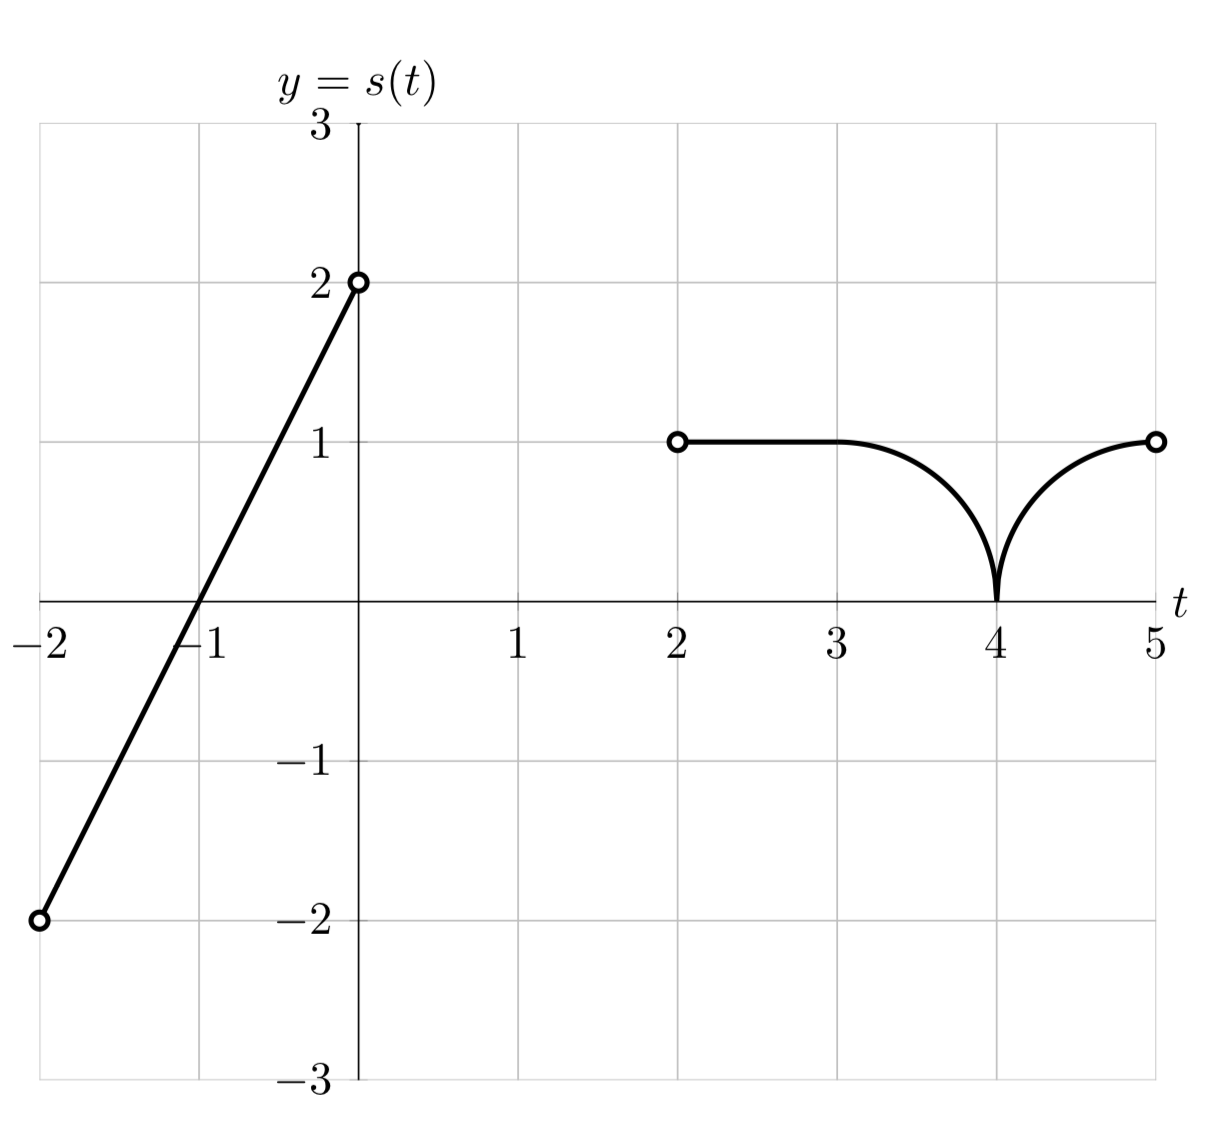
\includegraphics[scale=0.39]{graphs}
	
	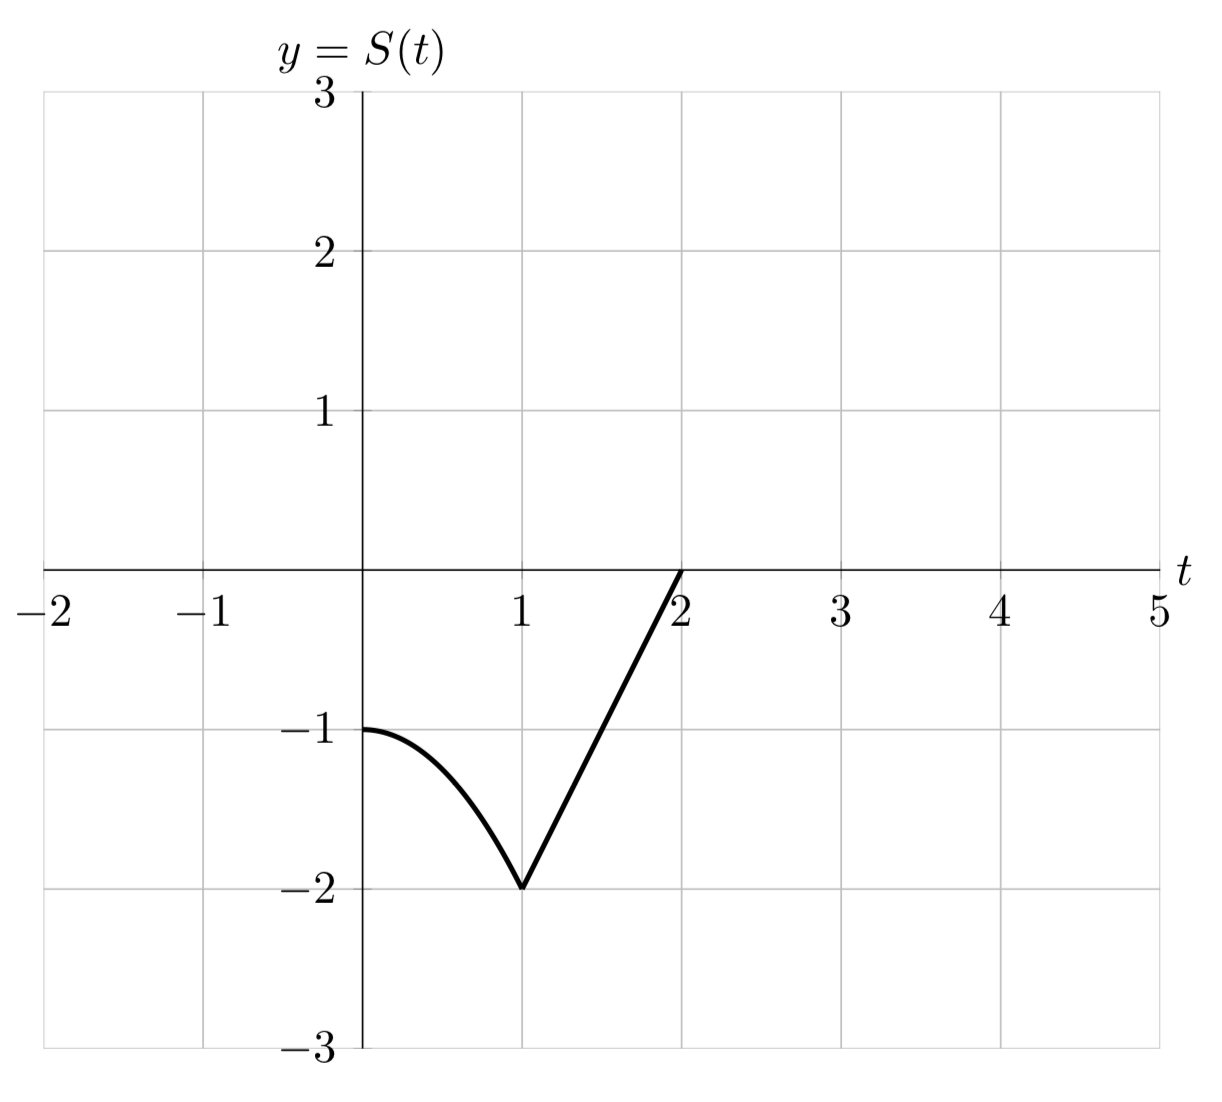
\includegraphics[scale=0.39]{Sgraph}
	\end{multicols}
	\begin{enumerate}[(a)]
		\item Use the portions of the graphs to fill in the exact values of $S(t)$ in the table below.
		$$\begin{array}{|c||c|c|c|c|c|c|c|}
	\hline
	t & -2 & -1 & 0 & 2 & 3 & 5 \\
	\hline
	S(t) & & & & & & \\
	\hline
	\end{array}$$
      \item Sketch the missing portions of both $s$ and $S$ over the interval $-2 < t < 5$. Pay attention to:
\begin{itemize}
\item the values of $S(t)$ from the table above;
\item where $S$ is and is not differentiable;
\item the concavity of the graph $y = S(t)$.
\item where $S$ and $s$ are increasing/decreasing/constant;
\end{itemize}
\end{enumerate}
\begin{solution}
See \href{https://dhsp.math.lsa.umich.edu/exams/115exam3/f17/s5.pdf}{https://dhsp.math.lsa.umich.edu/exams/115exam3/f17/s5.pdf}
\end{solution}
\vspace{-0.3cm}
\question (Winter 2016 Final Exam) % problem 10
Which of the following is an antiderivative of the function $f(x)= \cos(x)$? Circle all the correct options.
\begin{multicols}{3}
\begin{enumerate}[(a)]
	\item $\frac{\cos(x)}{2}$
	\item $\sin(x) + 5$
	\item $\cos \left( x - \frac{\pi}{2} \right)$
	\item $\ln \left( 3e^{\sin(x)} \right)$
	\item $19- \sin(x)$
	\item None of these
\end{enumerate}
\end{multicols}
\begin{solution}
 See \href{https://dhsp.math.lsa.umich.edu/exams/115exam3/w16/s10.pdf}{https://dhsp.math.lsa.umich.edu/exams/115exam3/w16/s10.pdf}
\end{solution}
\vspace{-0.3cm}
\question (Fall 2017 Final Exam) % problem 9
Which of the following is an antiderivative of the function $f(x)= \frac{1}{x} + \cos(x)$? Circle all the correct options.
\begin{multicols}{3}
\begin{enumerate}[(a)]
	\item $-\frac{1}{x^2} - \sin(x)$
	\item $\ln(5x)+ \sin(x)$
	\item $\ln(x) + \sin(x) - 20$
	\item $\ln \left( \frac{1}{x} \cos(x) \right)$
	\item $\frac{1}{x^2} + \sin(x)$
	\item None of these
\end{enumerate}
\end{multicols}
\begin{solution}
  See \href{https://dhsp.math.lsa.umich.edu/exams/115exam3/f17/s9.pdf}{https://dhsp.math.lsa.umich.edu/exams/115exam3/f17/s9.pdf}
\end{solution}
\end{questions}
\end{document}
%%% Local Variables:
%%% mode: latex
%%% TeX-master: t
%%% End:
